
\chapter{Species Diversification}

{\color{gray} \begin{fquote}[ Alan Turing]  Mathematical reasoning may be regarded rather schematically as the exercise of a combination of two facilities, which we may call intuition and ingenuity. \end{fquote} }



\section{The evolutionary diversification process and the mechanism behind it. Review and Research Questions.}

The mechanisms behind the variation in species diversity is one of the fundamental questions of evolutionary biology. Kendall \cite{kendall1948some} considered a convenient birth-death process, which can be recast in terms of speciation and extinction events, and thus represents an extension of the Yule process \cite{yule1925mathematical}. Considering $n_t$ as the number of species (of a related genus) at time $t$, the master equation for $n_t$ in presence of extinction and speciation can be written as  

 $$ \frac{dP(n_t)}{dt} = \lambda_{n_t-1}(n_t-1)P(n_t-1)+\mu_{n_t+1}(n_t+1)P(n_t+1)-(\mu_{n_t}+\lambda_{n_t})n_tP(n_t) $$


where $\lambda_n$ and $\mu_n$ are the per capita speciation and extinction rates, respectively, and $n_t$ the total number of species on moment $t$.\\

Based on this idea, the simplest and most widely applied of a variety of model is the random speciation-extinction process \cite{nee1994reconstructed}. In a random speciation-extinction process, both speciation and extinction have instantaneous probability, or rates ($\lambda$ and $\mu$) which determine the probabilities that a clade either splits or terminates within a given time interval. In a simple branching process, the expected number of a clade increases exponentially, that is 

\begin{equation}
 E(n_t) = n_0e^{(\lambda-\mu)t} 
\label{exp1}
\end{equation}

Despite this elegance, this approach is not realistic, evolutionary history of species is widely more complex:

\begin{itemize}

	\item Each branch in the growing tree might not have the same potential fate to speciate or to get extinct. In fact, in many cases depends on several characteristics of the species.
	 
	\item Ecological interactions are important.
	
	\item Geography, location and climate influence diversification of species.
	
	\item Evolution is likely to depend on diversity of species.
	
	\item Etcetera. 

\end{itemize} 


All this ecological factors needs to be considered if we want to build model consistent with real phylogenies; for example, typically we see a common slow down on diversification towards the present \cite{moen2014does} (but see \cite{jetz2012global}) which is the opposite equation \ref{exp1} predicts. Some biological explanations might underlie diversification slowdowns, like the protracted speciation model \cite{etienne2012prolonging}, but those models do not have, for instance, a geographical component. \\

Spatial-temporal factors as well as traits and diversity dependence are some of the ecological information we should include to consider realistic models, however, this complex scenario increase the dimensionality of the system enormously, rendering them practically intractable.  \\


% Reescribir esto
%On next section we will make a quick review of the mentioned ecological factors which are potentially evolved on the mechanism underlying biodiversity and the research questions we are interested on: \\
On next chapter we will describe a novel methodological contribution to this project which aims to produce a computational feasible and consistent model selection procedure, able to take in consideration all ecological variables mentioned above. On the remaining part of this chapter we formulate and discuss the research questions this project is going to analyze. Figure \ref{Diagrama} shows a Diagram of different factors we are interested to analyze as potential drivers of species diversification; on parenthesis we recognize the research questions related to these factors. \\



%It is important to claim that we are interested in deal with interactions between species
\begin{figure}
\centering
\begin{tikzpicture}
  \path [
    mindmap,
    text = white,
    level 1 concept/.append style =
      { sibling angle=90},
    level 2 concept/.append style =
      {font=\tiny\bfseries},
    level 3 concept/.append style =
      {font=\tiny\bfseries},
    tex/.style     = {concept, ball color=blue,
      font=\bfseries},
    engines/.style = {concept, ball color=green!50!black},
    formats/.style = {concept, ball color=purple!70!black},
    systems/.style = {concept, ball color=brown!90!black},
    editors/.style = {concept, ball color=orange!90!black}
  ]
  node [tex] {Diversification} [clockwise from=0]
    child[concept color=orange!50!blue, nodes={editors}] {
      node {Time (Q5)} [clockwise from=140]}	
    child[concept color=green!50!blue, nodes={engines}] {
      node {Enviroment (Q1, Q2,Q4)} [clockwise from=0]
        child { node {Climate} }
        child { node {Geography} }
        child { node {Location} }}
    child [concept color=purple!50!blue, nodes={formats}] {
      node {Traits (Q3, Q4)} [clockwise from=300]
        child { node {Etcetera} }
        child { node {Dispersal} }
        child { node {Diet} }
        child { node {Population} }
        child { node {Body size} }}
    child [concept color=brown!50!blue, nodes={systems}] {
      node {Ecological Interactions (Q1)} [clockwise from=110]
          child { node {Diversity} }
          child { node{Ecological limits} }};
\end{tikzpicture}
\caption{Representation of potential factors involved on species diversification we will include in the model. On parenthesis we see the associated research questions discussed on this chapter.}
\label{Diagrama}
\end{figure}



{\bf Q1:} Do species interaction determine diversification?\\

Species richness varies widely over the surface of the Earth \cite{ricklefs2007estimating} and patterns of species richness reflect the balance between speciation and extinction over the evolutionary history of life. Theories of how species evolve in changing environments  mostly consider single species in isolation or pairs of interacting species \cite{barraclough2015species}. \\

We are interested on the impact on interactions between species which happen locally, and therefore are hard to tackle. Reducing the complexity of the system we aim to incorporate a general approach to include species interaction on the diversification process. \\

An initial step would be to extend the approach of Etienne et al. \cite{etienne2011diversity}, which considers a caring capacity $K$ based on competition and the idea that ecological constrains place upper limits on regional diversity and that diversity is usually close to its limit \cite{cornell2013regional}. Thus, they assume that the speciation rate is limited to the caring capacity $K$ and therefore to the diversity of species $n$ 

$$ \lambda_n = \max (0, \lambda_0 - (\lambda_0 - \mu_n)\frac{n}{K} $$

We will generalize this approach considering the caring capacity $K(x)$ as a function of location $x \in \mathbb{R}^2$. Based on this, an important underlying analysis of this research question, would be to understand what is the shape of $K(x)$ as a function of location, or more generally,  the following question:\\

{\bf Q2}: How diversification rates and ecological limits varies across location?. \\


The next question is related to the impact of species' traits on diversification:\\


{\bf Q3:} Do different characteristics of species influence diversification? if yes, which ones and how they influence evolution? \\



The influence of species' traits on lineage diversification is an active area of macroevolutionary research, attributes of species, including population size, generation time, mechanism of pollination and seed dispersal, strength of sexual selection, body mass, longevity of species, diet in insects, latitude of birds and butterflies, sex allocation in flowering plants, and a large etcetera \cite{barraclough1998revealing}, has been studied and are still a matter of active research.  Sister clade comparison \cite{magallon2001absolute} has been a possible way to find relationship between traits and diversification rates, but approaches incorporating phylogenetic tree topology and the patterns of branching times had shown a greater statistical power because they incorporate more information about the patterns of diversification \cite{paradis2005statistical}. Among these methods we find models for binary-states traits \cite{maddison2007estimating},  quantitative and continuous traits \cite{fitzjohn2010quantitative}, multiple traits \cite{fitzjohn2012diversitree}, etc. But not a general approach where we can include all different kind of traits in a flexible way.


%Comparisons of species richness among sister clades enable one to test hypotheses about the influence of species attributes and environmental conditions, such as climate and landscape heterogeneity, on diversification \cite{paradis2005statistical}\\

Even though those methods have been successful finding important ecological insights in some way, they have some major drawbacks. For one side, most of the models require complete phylogenies, that is, extant specie must be present in a well-resolved phylogeny \cite{fitzjohn2009estimating}, but in reality information on extinct species is absent or, at best, incomplete; and this will never get better, simple collecting more data is not possible. For other side, even models which deals with incomplete data have a big constrain: they lack of flexibility, in the sense that they are able to be applied to very special cases, but not in a general framework, for any kind of trait. \\

It is important to note that the question Q3 is very general, and actually triggers many other research questions. For instance, dispersal is a life-history trait that influences the dynamics and persistence of populations, the distribution and abudance of species, and community structure \cite{silwood1999evolutionary}, we are also interested in their impact on evolution:\\

{\bf Q4}: What is the role of dispersal on evolutionary processes?\\



 

%We can see a decrease in diversity from its peak in the humid tropics towards higher latitudes \cite{hillebrand2004generality} \\

Finally, we would like to incorporate the temporal component on evolution as well. Several studies (e.g  \cite{rosindell2010protracted}) claim that is necessary to incorporate protracted speciation for a proper understanding of biodiversity, this makes us formulate the following question:\\


{\bf Q5}: Do we need to consider speciation as a protracted process? \\


In that way, our model should be flexible enough to incorporate protracted speciation, in the sense that it should also model speciation as a gradual process rather than an instantaneous one. \\

In this project we aim to build a general statistical framework able to incorporate any potential influential trait in a straightforward manner. Details of the methodology are described in next chapter. \\
\section{Incomplete Phylogeny trees}


A limitation of phylogenetic reconstruction based on extant species is that lineages are not represented (see Figure \ref{incomp}). This limitations makes estimating speciation and extinction rates problematic life \cite{ricklefs2007estimating}. As was mentioned before information of extinct species is usually absent or, at best, incomplete.  \\

The problem of missing data is widely considered to be the most significant obstacle in both, reconstructing phylogenetic relationships and modeling diversification process \cite{wiens2003missing}.  In this project, following Friedman et al. \cite{friedman2002structural} we will use a structural EM approach to tackle this problem efficiently. The procedure is described on next chapter.  



\begin{figure}
\centering
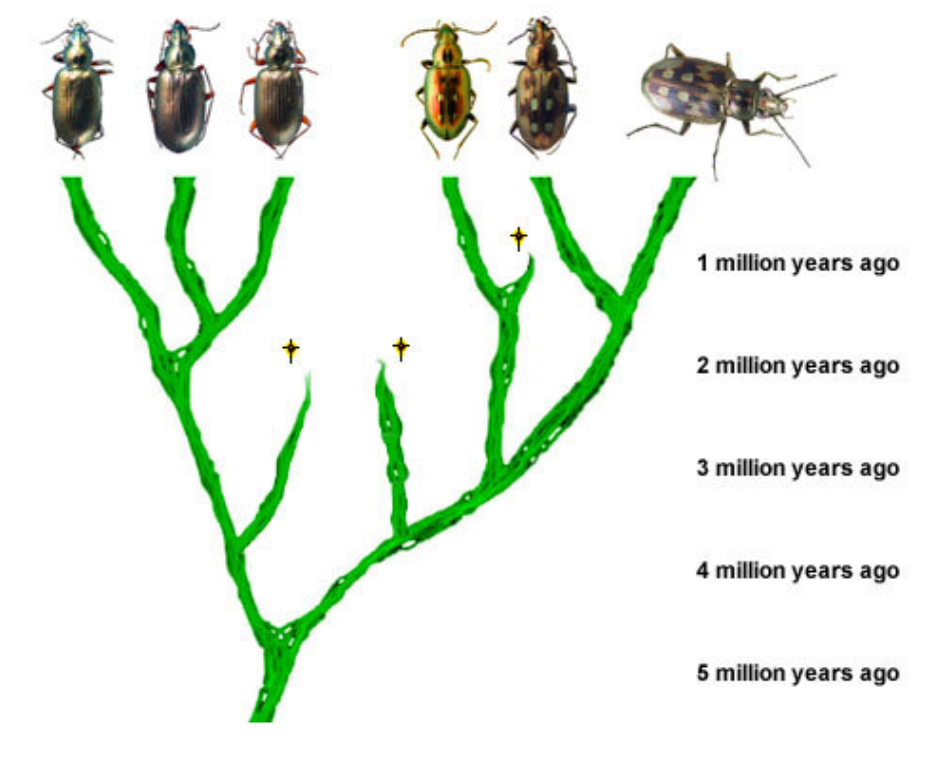
\includegraphics[scale=0.45]{Pictures/tree.png}
\caption{A phylogenetic tree of beach beetles of the genus \emph{Bembidion}. Some branches have gone extinct in the past, while others represent species living today.}
\label{incomp}
\end{figure}

